% !TeX spellcheck = fr-moderne
\section{Introduction de l'industrie de la télécommunication}
\subsection{L'evolution des normes de téléphonie mobile}
Depuis 1984, il y a déjà plusieurs standards ont été utilisés par les opérateurs dans le monde entier. Voici un tableau de différents standards de mobile en Europe et les paramétrés \ref{tbl:GMIE}. 
\begin{table}[H]
\begin{tabular}{|p{2cm}|p{2cm}|p{2cm}|p{4cm}|}
	\hline
	Génération&Acronyme&Description&Débit\\
	\hline
	1G		&Radiocom 2000	&Échanges de type voix uniquement&analogique\\
	\hline
	\hline
	2G		&GSM			&Échanges de type voix uniquement	&9,05 kbps\\
	\hline
	2,5G	&GPRS			&Échange de données sauf voix		&171,2 kbps / 50 kbps / 17,9 kbps\\
	\hline
	\hline
	3G		&UMTS			&Voix + données						&144 kbps rurale, 384 kbps urbaine, 1,9 Mbps point fixe / -\\
	\hline
	3.5G ou 3G+ ou H&HSPA	&Évolution de l'UMTS				&14,4 Mbps / 3,6 Mbps / -\\
	\hline
	\hline
	4G		&LTE			&Long Term Evolution (Données)				&150 Mbps / 40 Mbps / -\\
	\hline
	4G		&LTE-Advanced	&Long Term Evolution Advanced (Données+voix)		&1 Gbps à l'arrêt, 100 Mbps en mouvement / - / -\\
	\hline
\end{tabular}
\caption{Les différentes générations de téléphonie mobile en Europe}
 \label{tbl:GMIE}
\end{table}

\subsubsection{La première génération}
En télécommunication, \textsf{1G} est la première génération des standards pour la téléphonie mobile, Il s'agit de la première apparition du réseaux de téléphonie mobile. 1G consiste aux réseaux analogiques qui peuvent échanges de type voix uniquement.
\subsubsection{La deuxième génération}
\textsf{2G}, la technologie de téléphonie sans fil de deuxième génération, la différence entre les réseaux 1G et 2G est: les signaux radio sur les réseaux 1G sont analogiques, et ceux de 2G sont numériques.

Systèmes 2G ont été significativement plus efficaces du spectre permettant de bien plus grands taux de pénétration du téléphone mobile, en plus les données vocales numériques peuvent être compressées et multiplexées beaucoup plus efficacement que les codages de la voix analogique grâce à l'utilisation de codecs différents, ce qui permet plus d'appels à transmettre dans la même quantité de bande passante radio. Et 2G introduit pour la première fois le service de données pour mobile. La Technologie 2G permettent les divers réseaux de téléphonie mobile d'utiliser des services tels que le SMS et MMS. Tous les messages de texte envoyés au delà de 2G sont chiffrés numériquement, ce qui permet le transfert de données de telle sorte que seul le destinataire peut recevoir et lire.   

Réseaux 2G ont été construits principalement pour le service téléphonique et de transmission de données lente (défini dans les documents de spécifications IMT-2000).

Réseaux \textsc{2,5G}, qu'on les qualifie souvent de General packet Radio Service ou GPRS, est une norme pour la téléphonie mobile dérivée du GSM et complémentaire de celui-ci, permettant un débit de données plus élevé. Le 2,5 indique que c'est une technologie à mi-chemin entre le GSM (deuxième génération) et l'UMTS (troisième génération). Le GPRS est une extension du protocole GSM : il ajoute par rapport à ce dernier la transmission par paquets. Cette méthode est plus adaptée à la transmission de données. En effet, les ressources ne sont allouées que lorsque des données sont échangées, contrairement au mode « circuit » en GSM où un circuit est établi – et les ressources associées – pour toute la durée de la communication. Le GPRS a ensuite évolué au début des années 2000 vers la norme \textsc{edge} également optimisée pour transférer des données et qui utilise les mêmes antennes et les mêmes fréquences radio.

\subsubsection{La troisième génération}
La troisième génération (3G) des normes de téléphonie mobile. Elle est représentée principalement par W-CDMAmm, CDMA2000, TD-SCDMA et WiMAX. Elle permet des débits de 2 à 42 Mb/s qui sont bien plus rapides que la génération précédente. Grâce à l'utilisation des règles de classement d'utilisateurs, les bandes de fréquences supérieures rend la capacité du réseau augmenter.

Les différents standard  3G et ses prédécesseurs, utilisent le domaine CS (Circuit Switch)  pour le service vocal, et le domaine PS (Packet Switch) s'occupant du service de données \ref{fig:3G2}.
\subsubsection{La quatrième génération}
La quatrième génération des standards pour la téléphonie mobile, succédant à la 2G et la 3G, en théorie, elle permet de transmettre des données à des débits supérieurs à 100 Mb/s. 

Une des particularités de la 4G est sa EPC (Evolved Packet Core) basé sur IP, et il n'y a plus de mode commuté (le 'Circuit Switched Domain' qui s'occupe le service vocal dans les standard précédents), ce qui signifie que le service vocal transmis sur l'internet \ref{fig:4g}. 
\begin{figure}[H]
\centering
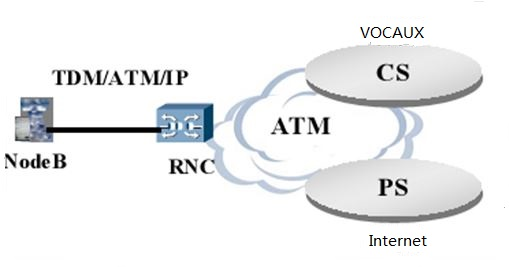
\includegraphics[width=0.7\linewidth]{images/3G2}
\caption{Réseau 3G et ses prédécesseur}
\label{fig:3G2}
\end{figure}
\begin{figure}[H]
\centering
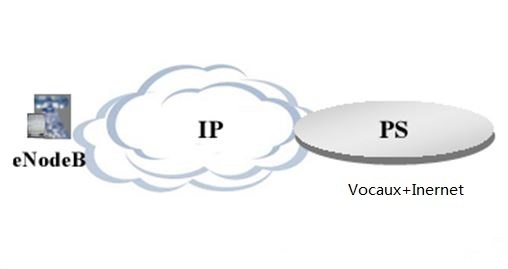
\includegraphics[width=0.7\linewidth]{images/4g}
\caption{Réseau 4G}
\label{fig:4g}
\end{figure}




Les avantages du réseau 4G sont:  plus haut débit, mieux utilisation de la bande de fréquence, moins de délai (délai dans le panneau de l'utilisateur est inférieur que 5 ms, délai dans le panneau de commande est inférieur que 100 ms ), plus simple structure du réseau, moins de consommation d'énergie terminale.

\subsection{Le réseau LTE}
Le LTE (Long Term Evolution) est l'évolution la plus récente des normes de CDMA 2000, TD-SCDMA, GSM. La technologie LTE est considérée comme une norme de troisième génération '3.9G', et la 'vraie 4G', appelée LTE-Advanced est reconnue par l'UIT comme une technologie 4G en 2010. LTE a deux branches: LTE-FDD (Frequency-Division Duplex  Long Term Evolution)et LTE-TDD, (Time Division Duplex Long Term Evolution)les deux standards sont similaires, la différence entre les deux standards est moins de 15\% \ref{evolution}. En 2011-2012, les réseaux LTE-TDD sont commercialisés sous l'appellation 4G par le CMCC en Chine.
      \begin{figure}[H]
          \centering
          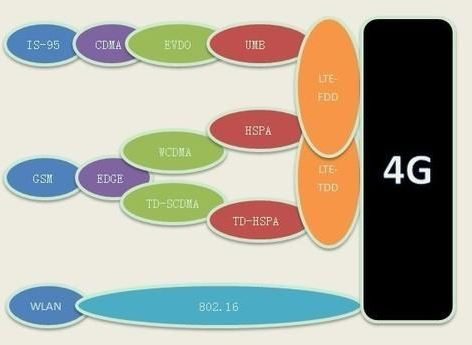
\includegraphics[width=4in]{images/evolution.JPG}
          \caption{l'evolution des standard}
          \label{evolution}
      \end{figure}
      
\subsubsection{La structure du réseau LTE}
Le réseau 4G contient 3 parties: UE( User Equipment);, eNodeB (les stations de base), EPC (Evolved Packet Core). EPC contient MME, S-GW, P-GW et HSS \ref{structure4G}  \ref{founction du chaque partie}. 
    
      \begin{figure}[H]
          \centering
          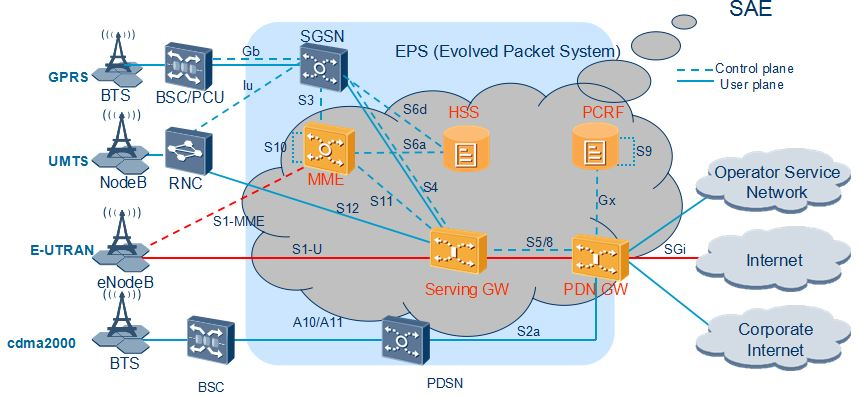
\includegraphics[width=5in]{images/enb2.jpg}
          \caption{la structure du réseau}
          \label{structure4G}
      \end{figure}
      
\begin{table}[H]
	\begin{tabular}{|>{\centering\arraybackslash}p{2cm}|>{\centering\arraybackslash}p{11 cm}|}
		\hline Part &                     Fonction\\
		\hline MME & 
			L'authentification des utilisateurs et la gestion des clés,  Cryptage de la couche NAS,  Gestion de la liste TA, Sélection P-GW ou S-GW \\ 
		\hline Service Gateway & Compression d'en-tête IP, Routage de paquets et la transmission, La commutation entre eNB, Facturation des utilisateurs porteur \\ 
		\hline PDN Gateway & L'allocation des adresses IP de UE, l'accès aux fonction de gestion de réseau externes, Facturation en service \\ 
		\hline HSS(Home Subscriber Service) & Stockée données de l'utilisateur associées au service \\ 
		\hline PCRF & Roaming \\ 
		\hline 
	\end{tabular} 
	\caption{la fonction du chaque partie}
	\label{founction du chaque partie}
\end{table}    

Entre deux \textsc{e-utrans}, il y a l'interface X2, l'interface S-11 se trouve entre S-GW et MME, \textsc{e-utran} et S-GW échangent les données par l'interface S1-U et il échange les donnée par l'interface S1-AP avec MME, MME et HSS utilisent l'interface S6A, et l'interface S5/8 entre S-GW et P-GW, Gx entre PCRF et P-GW. En mettant des capteurs sur les interfaces, les opérateurs et les fournisseurs d'équipement peuvent collecter les données de signalisation, et utilisent ces informations pour trouver les défauts du système. 

\begin{figure}[H]
\centering
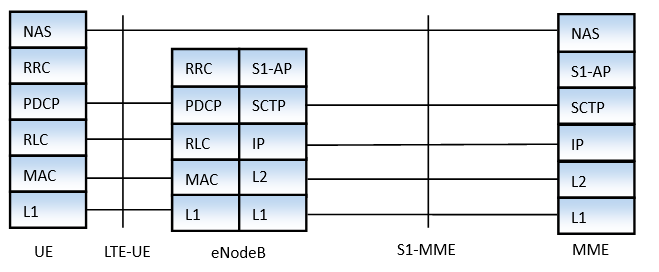
\includegraphics[width=0.9\linewidth]{images/s1-mme}
\caption{Contrôle plan}
\label{fig:s1-mme}
\end{figure}

\begin{figure}[H]
\centering
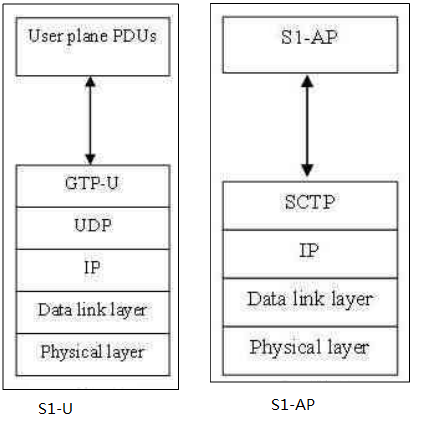
\includegraphics[width=0.9\linewidth]{images/S1-U}
\caption{User plan}
\label{fig:S1-U}
\end{figure}


\section{Les solutions existantes}

L'optimisation du service téléphonique est très importante. L'opérateur a construit un immense réseau de télécommunication, mais à cause de la mauvaise configuration du système, les utilisateurs ne sont pas satisfaits avec les services, les investissements n'ont pas été remis. Donc les entreprises comme IBM, Huawei, et d'autres fournisseurs du équipement essaient de trouver la meilleure solution. 

Maintenant, il y a beaucoup des gens qui travaillent dans ce domaine, nous avons trouvé beaucoup d'articles sur l'optimisation du réseau télécommunication, mais les articles sont basés sur réseau 3G ou 2G. 

Il y a trois techniques qui sont beaucoup utilisées:
\begin{enumerate}
\item \textsf{la Technique KQI};
\item \textsf{la Technique QoE};
\item \textsf{la Technique qui étude les comportements de l'utilisateur}.
\end{enumerate}

\subsection{la Technique KQI}:

La technique le plus souvent utilisée s'appelle 'KQI' ( Key Quality Indicator) \ref{fig:kqi}, cette méthode a été beaucoup utilisée. Et cette technique peut généralement divisé en deux étapes. D'abord, nous devons calculer le score de KPI, pour calculer le KPI en premier, il faut analyser le processus d'un service et choisir les indicateurs de performance. Ensuite, nous pouvons calculer le score d'un processus en utilisant une équation linéaire, le poids de chaque attribut change selon le service, par exemple, pour le service SMS, le délai porte peu d'importance, mais le délai du service est important pour le service HTTP. \textsc{à} la fin, nous pouvons calculer le KQI avec les KPI \cite{kqi}. Mais les poids sont définis par les experts, et les valeurs peuvent être fausses ou pas précises. Et par fois le score est bon mais l'expérience de l'utilisateur n'est pas bonne.
\begin{figure}[H]
\centering
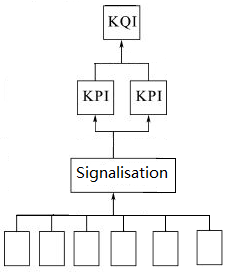
\includegraphics[width=5cm]{images/kqi}
\caption{KQI}
\label{fig:kqi}
\end{figure}

\subsection{la Technique QoE}:

KPI est un des indicateurs de qualité axés sur les performances du réseau, mais il ne reflète pas directement l'expérience de la qualité de service de l'utilisateur, parce que les expériences de l'utilisateur sont difficile à mesurer. Donc la technique QoE a été inventé. QoE défini la performance de la qualité de service et l'expérience de l'utilisateur de l'ensemble du réseau à partir de l'utilisateur.

Les utilisateurs ont nombreuses exigences pour les services téléphoniques, Elles peuvent être résumées en deux aspects: la fiabilité et le confort. La fiabilité fait référence à l'activité de l'accessibilité, la disponibilité et la durabilité. Le confort est une qualité de service, un indice de la perception directe de l'utilisateur, qui dépend de l'expérience de l'utilisateur\cite{QoE}. Les relations entre QoE et QoS KPI sont: la fiabilité du service \ref{table.fiabilité}, le confort du service\ref{table.confort}. 

\begin{table}[H]
	\centering
	\caption{Fiabilité du service }
	\label{table.fiabilité}
\begin{tabular}{|c|c|}
\hline \rule[-2ex]{0pt}{5.5ex} KQI & QoE \\ 
\hline \rule[-2ex]{0pt}{5.5ex} Accessibilité & Taux de succès  \\ 
\hline \rule[-2ex]{0pt}{5.5ex} Disponibilité  & Temps d'accès aux services \\ 
\hline \rule[-2ex]{0pt}{5.5ex} Durabilité & La durée de l'accès des services \\ 
\hline 
\end{tabular} 
\end{table}

\begin{table}[H]
	\centering
	\caption{Confort du service}
	\label{table.confort}
\begin{tabular}{|>{\centering\arraybackslash}p{5 cm}|>{\centering\arraybackslash}p{6 cm}|}
\hline KQI & QoE \\ 
\hline  & Taux de perte de paquets de couche d'application \\ 
\hline  & Le débit moyen  \newline \\ 
\hline La qualité du service de transmission & Stabilité de la transmission \\ 
\hline & Le bout en bout délai moyen \newline  \\ 
\hline & Gigue \newline  \\ 
\hline Le persistant de la connexion de service & La vitesse et la difficulté du service d'assistance\\ 
\hline 
\end{tabular} 
\end{table}

Maintenant, la technique de QoE a été beaucoup utilisée pour le service vocal. Et à cause de la complexité du service de données, il n'y a pas un standard de QoE pour le service de données. 

En utilisant la technique KQI et QoE, nous pouvons mesurer la qualité du service, les résultats peuvent aider les opérateurs trouver les services de mauvaise qualité, les opérateur peuvent améliorer les services selon le résultat, finalement améliorer la notation de l'utilisateur.  

Le résultat de KQI dépend seulement des performances du réseau, donc nous avons besoin des informations et des performances de réseau. Et la technologie QoE a besoin du résultat de KQI et de feed-back de l'utilisateur, le feed-back peut être obtenu par l'enquête ou les plaintes des utilisateurs et par les mesures directs.

\subsection{la Technique qui étude les comportements de l'utilisateur} 

Aussi il y a un groupe qui utilise les comportements de l'utilisateur pour définir la qualité du service\cite{UB}. Le groupe utilise cette méthode dans le service vocal, il cherche la situation où l'utilisateur accroche et ré-appel le même personne. \textsc{à} la fin, cette méthode aide l'opérateur corriger le paramètre d'erreur.

Selon l'article, cette méthode peut aider l'opérateur trouver les défauts du système, mais il a nombreuses restrictions, par exemple, nous ne pouvons pas utiliser cette technologie dans le service de SMS, etc.



\section{Le présentation de notre solution}

La méthode qui utilise les comportements de l'utilisateur est intéressante, mais nous trouvons qu'elle peut utiliser seulement dans le service vocal, nous n'avons pas trouvé les règles similaires dans l'autre service. D'ailleurs, le réseau LTE ne support pas le service vocal, donc il n'existe pas d'optimisation du service vocal dans le réseau LTE et nous n'avons pas de données. Donc nous ne pouvons pas utiliser cette méthode.

La technique QoE et KQI sont beaucoup utilisés, mais d'abord, pour la méthode QoE, nous avons besoin des réponses des utilisateurs, mais nous n'avons pas assez de temps, et des raisons financières, le CMCC ne peut pas nous fournir ces données. Et l'équation qu'on utilise pour calculer KPI n'est pas convaincante, voici une exemple d'un équation pour calculer la disponibilité du réseau pour le service SMS dans réseau 3G\ref{fig:kpi}. 
\begin{figure}[H]
\centering
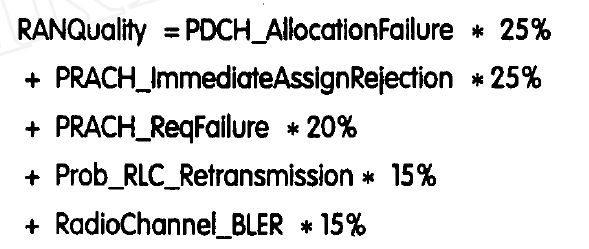
\includegraphics[width=0.7\linewidth]{images/kpi}
\caption{Un exemple d'un équation pour calculer la disponibilité}
\label{fig:kpi}
\end{figure}

Le poids du chaque attributs est défini par les experts, Mais l'utilisateur n'est pas satisfait du service. Nous croyons que l'erreur a été causée par l'inexacte équation, et nous pensons que les algorithmes de classification peuvent aider à améliorer le résultat, mais très vite nous avons trouvé que le CMCC ne peut pas nous fournir ce type de données. Sans la connaissance à priori, nous ne pouvons pas utiliser ces algorithmes. Nous avons aussi pensé à utiliser le externalisation ouverte (crowdsourcing), à notre avis si le CMCC peut lancer un projet de externalisation ouverte. Si le CMCC peut encourager ses utilisateurs donner les notes aux services pour obtenir des crédits, nous pouvons obtenir la connaissance à priori, et à l'aide de ces données, nous pouvons trouver une équation peut-être mieux que les équations écrivent par les experts. Mais bien sur, le CMCC n'a pas accepté cette idée, parce que cette méthode peut coûter cher, et peut-être il n'y a pas de revenu direct. Et l'entreprise ne fait pas de l'investissement sans retour. Donc nous n'avons pas de connaissance a priori.

Finalement, nous avons décidé d'utiliser la technique de l'apprentissage non supervisé, il contient la notion de Réseau de neurones et l'algorithme de clustering etc. Nous avons choisi l'algorithme de clustering. Et nous avons utilisé la technique de l'arbre couvrant de poids minimal en anglais Minimum spanning tree \textsf{(MST)} et la méthode \textsf{Règles d'association} et \textsf{PCA}.

\subsection{Clustering}
L'algorithme de clustering est une des méthodes de classification non supervisée. Il est beaucoup utilisé quand la donnée n'a pas de connaissance a priori.

C'est une méthode statistique d'analyse des données. Elle divise un ensemble de données en différents groupes, les données de chaque groupe est mathématiquement plus proche que les données de l'autre groupe,  et nous supposons que les données dans le même partition ont des caractéristiques similaires.

Il existe de multiples méthodes de regroupement des données, parmi lesquelles:
\begin{itemize}
\item Classification basées sur la densité;
\item Classification hiérarchique;
\item Classification par partitionnement;
\item Classification par grille;
\item Classification basées sur des modèles.
\end{itemize}
\vspace{1ex}

Les étapes de cette algorithme est:
\begin{itemize}
\item Choisir $k$ points qui représentent la position moyenne des $k$ partitions initiales (au hasard) ;
\item Répéter les étape suivant jusqu'à convergence :
\begin{enumerate}
\item assigner chaque observation à la partition la plus proche
\item mettre à jour la moyenne de chaque cluster
\end{enumerate}
\end{itemize}
\begin{figure}[H]
\centering
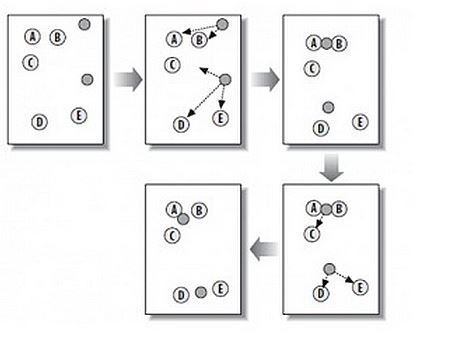
\includegraphics[width=0.7\linewidth]{images/kmeans}
\caption{étapes de l'algorithme K-Means}
\label{fig:kmeans}
\end{figure}

Nous avons utilisé l'algorithme K-Means et CLARA (Clustering Large Applications ). Ils sont deux techniques de Classification par partitionnement.

Le but de cet algorithme est de diviser des données en K partitions (clusters) dans lesquelles les données appartient à la partition avec la moyenne la plus proche. 

\subsubsection{La distance}

Quand on regroupe un ensemble de données, on calcule la distance entre chaque échantillon, la distance entre les échantillons dans un même groupe est plus petite que les échantillons dans l'autre groupe. on suppose que pour les deux échantillons les plus similaires , plus la distance est petite.


Il y a plusieurs moyens de calculer la similarité. On utilise la technique qui est basée sur la distance Les techniques utilisés le plus souvent sont: \emph{distance euclidienne}, \emph{distance de Hamming}, \emph{distance Manhattan}, etc. Aussi il existe des méthodes qui mesurent la similarité, y compris: \emph{coefficient de Jaccard}, \emph{cosinus similarité}, etc . Nous décidons de utiliser la distance euclidienne pour calculer la similarité.

$$d(x,y) = \sqrt {\sum_{k=1}^n  (x_{k}-y_{k})^2}$$

$n$ est la dimension, $x_{k}$ et $ y_{k}$ sont le k-ème attributs de échantillon x et y.


\subsubsection{La validité de clustering}
Cette méthode a été utilisée dans beaucoup de différents domaines. Mais la qualité du résultat dépend du nombre de clusters ou de la valeur de K, différents paramètres peuvent mener à des résultats très différents.

En 1974, Mme \textsc{Bezdek} a proposé cette question de d'évaluation, et donné la première fonction pour évaluer le résultat du clustering: \textsf{Partition}  \textsf{Coefficient}. Par la suite, de nombreux chercheurs ont proposé une variété de fonctions pour évaluer le résultat, et évaluer les qualités et le champ d'application de ses fonctions. 

Par mesure de l'efficacité entre les partitions et inter-partition, on peut évaluer le clustering. Le résultat de clustering idéal devrait être l'obtention de la distance minimale dans les partitions, et la distance maximale entre les partitions. C'est à dire avec le plus petit cohésion dans la partition, et le plus élevé degré de la séparation entre les partitions. La cohésion mesure le degré de proximité dans le groupe, et la séparation mesure le degré de dissimilarité entre les groupes. La cohésion et la séparation peuvent être calculée par les équations suivantes.

$$cohésion(C_{i}) = \sum_{x\in1} proximity(x, c_{i})$$

$$séparation(C_{i},C_{j}) = proximity(c_{i}, c_{j})$$


Dans les formules, le \(c\)\ est le centre de gravité d'une partition, \(proximity(a,b)\)\ est la mesure de proximité entre la partition a et b.

Le degré de la cohésion de clusters et celui séparation sont souvent utilisés comme une mesures principales pour évaluer le résultat de clustering. Un bon regroupement devrait être à la fois un petit degré de la cohésion et un grand degré de la séparation.

Le degré de la cohésion et celui de la séparation de la partition ne sont pas indépendants, la somme des deux est une constante, on suppose que quand on a le minimal degré de la cohésion, on peut avoir le maximal degré de la séparation. \textsc{é}videment, nous devons utiliser à la fois le degré de la cohésion et celui séparation pour mesurer la qualité du regroupement.

\subsubsection{La silhouette C\oe fficient}

Kaufman a proposé la silhouette c\oe fficient en 2010, cette méthode utilise à la fois les deux degrés.

\begin{enumerate}
\item la silhouette c\oe fficient d'un échantillon:\\

 Pour un échantillon $d_{i}$, en supposent qu'il est dans groupe A, la silhouette c\oe fficient peut être calculée par cette formulaire:
$$s_{i}=\frac{b_{i}-a_{i}}{max(a_{i},b_{i})} $$

\emph{$a_{i}$ est la dissemblance moyenne de la donnée i avec toutes les autres données dans le même cluster(plus la valeur est petite, meilleur est le regroupement). $b_{i}$ est la différence moyenne de $i$ à tout autre groupe $i$ n'est pas un membre.}
\vspace{1ex}

Qui peut être écrite comme:
$$  s_{i}=\left\{
\begin{array}{rcl}
1-\frac{a_{i}}{b_{i}},       &      & if\  a_{i}<b_{i}\\
0,     &      & if\ a_{i}=b_{i}\\
\frac{b_{i}}{a_{i}}-1,     &      & if\ a_{i}>b_{i}\\
\end{array} \right. $$

D'après la définition ci-dessus, il est clair que la valeur de $s_{i}$ est entre $1$ et $-1$
$$-1<s_{i}<1$$

Pour que $s_{i}$ soit proche de $1$, nous demandons que le $a_{i}$ est plus petit que $b_{i}$. Comme $a_{i}$ mesure la dissemblable de i et son propre groupe, une petite valeur signifie qu'il est bien adapté. En outre, un grand $b_{i}$ implique que i est mal adapté à son groupe voisin. Ainsi, un $s_{i}$ près de $1$ signifie que la donnée est concentrée de manière appropriée. Si la valeur de $s_{i}$ est proche de $-1$, selon la même logique, nous voyons que la donnée $i$ serait plus appropriée si elle a été regroupée dans son groupe voisin.

\item la silhouette c\oe fficient moyenne:

Pour le résultat d'un regroupement, le silhouette c\oe fficient égale à:
$$s_{k}=\frac{1}{n}\sum_{i=1}^n s_{i}$$
\emph{$n$ est le nombre de données, $k$ est le nombre de partitions, $s_{k}$ est la moyenne de la silhouette c\oe fficient. Nous pouvons utiliser $s_{k}$ pour évaluer la qualité du clustering.}
\newline
\newline
Le $s_{i}$ est la moyenne sur l'ensemble des données d'un cluster, il est une mesure de degré de cohésion de toutes les données du cluster. Ainsi, les moyenne de $s_{i}$ de l'ensemble des données ($s_{k}$) est une mesure de la façon appropriée des données qui ont été regroupés. S'il y a trop peu de clusters, cela que peut se produire lorsque un mauvais choix de k est utilisé dans l'algorithme K-Means, la silhouette C\oe fficient de certains  groupes sera beaucoup plus petit que les autres. Donc la plot de silhouette C\oe fficient et la valeur moyenne de silhouette peuvent être utilisées pour déterminer le nombre de clusters (la valeur de $k$ ) optimaux pour le ensemble de données.
\end{enumerate} 

Après avoir trouvé les paramètres optimaux, nous pouvons utiliser l'algorithme clustering, et après avoir étudié et comparé les caractéristiques de chaque partition, nous pouvons définir la quelle partition qui représentent la mauvaise qualité de service. Le résultat peut nous aider à classifier le service. 

\subsection{Règles d'association}
La règle d'association est une méthode populaire, elle étudie le données d'une manière approfondie. Le but est de découvrir des relations ayant un intérêt pour le statisticien entre les variables. En se basant sur le concept de relations fortes, Rakesh Agrawal et son équipe présentent des règles d'association dont le but est de découvrir des similitudes entre des produits dans des données saisies sur une grande échelle dans les systèmes informatiques des points de ventes des chaînes de supermarchés. Par exemple, une règle découvre que si un homme achète les serviettes de bébé, il est susceptible de d'acheter les bières. Une telle information peut être utile quand on veut prendre des décisions marketing.

Les règles d'association sont employées aujourd'hui dans plusieurs domaines, incluant: la fouille du web, la détection d'intrusion et la bio-informatique.  Dans ces domaines, ils utilisent les données booléennes pour trouver les règles utiles. Mais dans le domaine télécommunication, les données de signalisation sont les données numériques. Donc nous ne pouvons pas directement utiliser la règles d'association. Par contre, nous pouvons convertir les données de type numérique en données de caractère en divisant les données dans plusieurs partitions \cite{AR}. Par exemple, nous avons des données numériques entre $0$ et $100$, et on divise les données en 10 partitions, donc les chiffres entre $0$ et $10$ peuvent présenter par $0<x<10$. En utilisant cette technique, nous pouvons utiliser la règle d'association pour trouver les relations dans les données.

 Il y a plusieurs méthodes pour diviser les attributs numériques: par catégorisation, l'analyse typologique, par analyse de l'histogramme, l'analyse basé sur l'entropie de discret, partition naturelle et ainsi de suite. 
 
 Nous décidons de utiliser le K-Means d'abord. Après avoir analysé le résultat, nous pouvons utiliser l'algorithme règles d'associations à l'aide du résultat de K-Means.

\subsection{K-Means et l'arbre couvrant de poids minimal }
D'après les techniques précédant, nous avons utilisé l'arbre couvrant de poids minimal avec K-Means.

En théorie des graphes, étant donné un graphe non orienté connexe dont les arêtes sont pondérées, un arbre couvrant de poids minimal de ce graphe est un arbre couvrant (sous-ensemble qui est un arbre et qui connecte tous les sommets ensemble) dont la somme des poids des arêtes est minimale\ref{fig:mst}. L'arbre couvrant de poids minimal est aussi connu sous certains autres noms, tel qu'arbre couvrant minimum ou encore arbre sous-tendant minimum. L'algorithme de Prim et l'algorithme de Kruskal sont deux méthodes classique, qui sont tous les deux l'algorithme glouton. 

\begin{figure}[H]
\centering
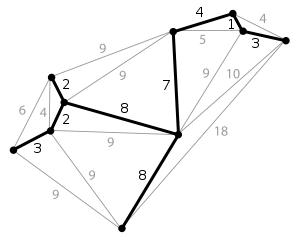
\includegraphics[width=0.5\linewidth]{images/mst}
\caption{MST}
\label{fig:mst}
\end{figure}

En coupant $C-1$ arêtes le plus grand, nous pouvons grouper le données en $C$ parties\ref{fig:mstc}.
\begin{figure}[H]
\centering
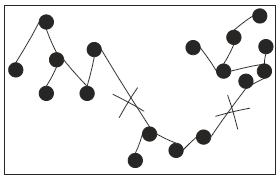
\includegraphics[width=0.4\linewidth]{images/mstc}
\caption{MST clustering}
\label{fig:mstc}
\end{figure}

Dans notre projet, nous avons choisi l'algorithme Prim et K-Means pour faire le clustering. 

La complexité de algorithme Prim est: $O((V+E)+\lg (V) = O(E \lg (V)) $, $V$ est l'ensemble de vertex ,$E$ est l'ensemble de arêtes.

La complexité de algorithme K-Means est: $O(nkt)$, $n$ est la quantité de données, $k$ est le nombre de partitions, t est le nombre d'itérations.
\subsubsection{L'algorithme KmMST}

Dans l'article \cite{KmMst}, nous avons trouvé une algorithme qui utilise K-Means et la MST. 

Parce que K-Means peut trouver des partitions sur forme sphéricité, et la valeur de $K$ n'est pas grand donc le résultat est influencer par les donnée de bruits, donc le résultat de K-Means est par fois peu satisfaisant. 

D'après l'article, nous pouvons choisir une grand valeur pour K, plus utilise la technique MST pour combiner les partition en C groupes en coupant C-1 arête. La performance est mieux que celui de K-Means\ref{fig:kmmst}.
\begin{figure}[H]
\centering
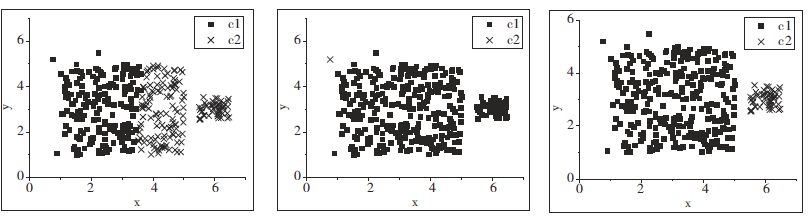
\includegraphics[width=1.0\linewidth]{images/kmmst}
\caption{La performance de K-Means, MST et KmMST}
\label{fig:kmmst}
\end{figure}

L'algorithme KmMST peut décrire comme suit:


\begin{enumerate}
\item calcule la valeur de $K$, $k=\left\vert n^r \right\vert \quad  \left( r \in \left[ 0,1 \right]  \right) $ par défaut la valeur de $r$ égale à $0,5$;
\item utilise l'algorithme K-Means, trouve K partitions;
\item calcule la distance entre chaque centre de la partition;
\item utilise l'algorithme Prim pour crée l'arbre couvrant de poids minimal;
\item coupe le $C-1$ plus bords qui ont le plus grand distance, le $C$ sous-graphe est le résultat de clustering.
\end{enumerate}


Pour utiliser cette algorithme, nous avons besoin: la quantité $n$ de données, le c\oe fficient de $r$ et la valeur de $C$. En utilisant cette méthode nous pouvons trouver les partitions.

\section{La mise en \oe uvre}
\subsection{Le logiciel utilisé}
L'objectif de notre projet est de trouver une méthode qui peut s'implanter dans les serveurs du CMCC, et aider le CMCC améliorer la qualité du réseau. D'après le directeur du R\&D département du CMCC, au total, CMCC a $20Pb$ de données stock dans ses base de données, donc le logiciel doit être capable d'exécuter grande quantité de données. En plus,  au lieu d'utiliser directement les logiciels comme SQL (qui n'est pas très efficient si on a beaucoup de données stock dans différents serveurs), le CMCC utilise 'Hadoop' pour stocker et gérer ses données.

Donc le logiciel que nous utilisons doit être capable d'exécuter grand quantité de données et peut travailler avec Hadoop. 

Finalement nous décidons de utiliser le langage \textsf{R}. Les avantages de R sont:

\begin{itemize}
\item R est un langage et un environnement pour le calcule statique et les graphiques; 
\item R offre une grande variété de statistiques (modélisation linéaire et non linéaire, classification, clustering, etc,) et des graphiques techniques, et il est très extensible ;
\item R est facile à utiliser; 
\item R est un logiciel libre, il compile et fonctionne sur une grande variété de plates-formes UNIX et les systèmes similaires (y compris FreeBSD et Linux), Windows et Mac OS;
\item en utilisant les packages fournis par 'Revolution Analytics', nous pouvons utiliser Hadoop en R.
\end{itemize}

Nous utilisons \textsf{Rstudio} comme notre environnement de programmation. C'est une interface d'utilisateurs puissante et productive pour R.

\subsection{Introduction des données}
%\,\up{\cite{specifi}}
Après quelque semaines de discussions avec les employés de différents départements de CMCC, ils nous ont fourni deux versions de données, et leurs spécifications du format\cite{specifi}. Nous avons trouvé que le CMCC n'a pas d'accès direct aux données, et le fournisseur d'équipement a modifié la spécification fournie par le CMCC, et il y a des erreurs dans les données fournies par le fournisseur d'équipement.

Ils nous ont envoyé $11$ dossiers, chaque dossier correspond à un service. les services sont 'rtsp', 'dns','mail', 'ftp', 'http-wap', 'mms', 'p2p', 'realtimecom', 'VoIP' et les données de signalisation entre \textsc{e-utran} et MME 'S1AP-NAS'.
    
Et nous avons trouvé que pour les services comme 'VoIP' et 'RTSP', ils ont très peu de données \ref{table.nombre}. Donc nous avons décidé d'utiliser le donnée du service 'HTTP'.

\begin{table}[H]
\centering
	\begin{tabular}{|>{\centering\arraybackslash}p{4 cm}|>{\centering\arraybackslash}p{4 cm}|}
	\hline \textsf{L'interface }& \textsf{Nombre de ligne} \\ 
	\hline S1-AP & $240$ \\ 
	\hline RTSP &$ 35$ \\ 
	\hline DNS  & $272562$ \\ 
	\hline Maill & $44$ \\ 
	\hline FTP &$ 71$ \\ 
	\hline HTTP-WAP & $50854$ \\ 
	\hline MMS & $193$ \\ 
	\hline P2P & $515$ \\ 
	\hline Realtimecom & $2082$ \\ 
	\hline S1U &$ 89759$ \\ 
	\hline VoIP & $28$ \\ 
	\hline 
	\end{tabular} 
	\caption{les dossiers de données}
	          \label{table.nombre}
\end{table}


Le dossier du service HTTP a $18,4Mbit$ , il y a $50854$ lignes, tous les données sont collectées par les capteurs placés entre les Service-Gateway et les eNodeB. Le capteur enregistre une ligne de données quand un processus est fini. Chaque ligne a $76$ attributs\ref{Fig.HTTP}.

      \begin{figure}[H]
          \centering
          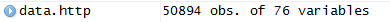
\includegraphics[width=3.5in]{images/http.png}
          \caption{les données du service HTTP}
          \label{Fig.HTTP}
      \end{figure}
      
Il contient des informations d'un UE (IMEI, IMSI, etc), les trafics de la liaison montante et la liaison descendante et le temps, l'adresse IP de UE, eNodeB et S-GW, le port de l'eNodeB et le S-GW, le délai du service, le site web, cookie, et aussi le temps de commencer et le temps d'arrêter.
Les données sont collectées dans $20.92$ minutes \Ref{fig:lasttime}.

      
      \begin{figure}[H]
\centering
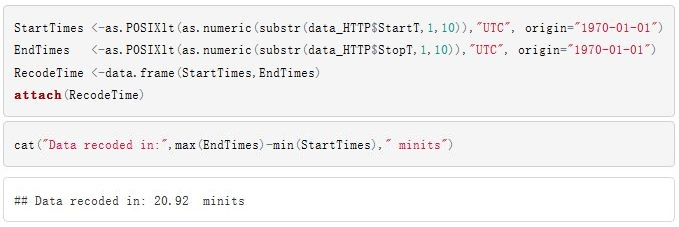
\includegraphics[width=15Cm]{images/lasttime}
\caption{Les données sont collectent dans 20.92 minutes}
\label{fig:lasttime}
\end{figure}

\subsection{Pré-traitement de données}
En analysant des données, nous avons trouvé des erreurs de données, et le fournisseur nous a confirmé que ces sont les défauts de leur système 4G. Pour les attributs 'IMSI', 'IMEI', 'MSISDN', $90$ \% de lignes sont vides, pour ceux qui ne sont pas vides, les contenus sont illisibles, et peuvent provoquer des erreurs de lecture \ref{fig:errorData}. Et nous avons trouvé que les contenus de certains lignes sont bizarres. 
\begin{figure}[H]
	\centering
	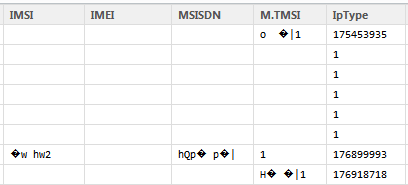
\includegraphics[width=0.7\linewidth]{images/errorData}
	\caption{erreur du codage BCD}
	\label{fig:errorData}
\end{figure}
Dans ce processus, le 'Down Link Online Time' égale à  $0$ ms , mais il a téléchargé $746$ bits, c'est clairement une erreur dd données.
\begin{figure}[H]
	\centering
	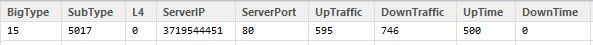
\includegraphics[width=0.9\linewidth]{images/bizarre}
	\caption{Erreur de la donnée}
	\label{fig:bizarre}
\end{figure}

 Nous avons décidé de ne pas utiliser les données avec ce type d'erreurs, à la fin, en supprimant ses données, il nous reste $37865$ lignes ($50894$ lignes en origine, $13029$ lignes ont été supprimé)  \ref{fig:newdata}.
 
\begin{figure}[H]
	\centering
	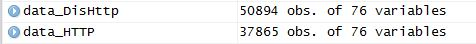
\includegraphics[width=0.8\linewidth]{images/newdata}
	\caption{Pré-traitement des données}
	\label{fig:newdata}
\end{figure}

Entre ces 76 attributs, une grande partie de ces informations sont inutiles, et pour certains attributs les contenus égalent tous à 0. Finalement, nous avons trouvé 11 attributs. ils sont:
\begin{table}[H]
\centering
\begin{tabular}{|>{\centering\arraybackslash}p{3 cm}|>{\centering\arraybackslash}p{3 cm}|>{\centering\arraybackslash}p{3 cm}|}
\hline \rule[-2ex]{0pt}{5.5ex} Signalisation & Signalisation & KPI \\ 
\hline \rule[-2ex]{0pt}{5.5ex} trafic en liaison montante & le temps en ligne & vitesse \\ 
\hline \rule[-2ex]{0pt}{5.5ex} trafic en liaison descendante  & le temps en ligne & vitesse \\ 
\hline \rule[-2ex]{0pt}{5.5ex}  & Http First Response Time & délai \\ 
\hline \rule[-2ex]{0pt}{5.5ex}  & Http Last Packet Time & délai \\ 
\hline \rule[-2ex]{0pt}{5.5ex}  & Http Last Ack Time & délai \\ 
\hline \rule[-2ex]{0pt}{5.5ex}  Packet Num en liaison montante & retransmission de paquets Num en liaison montante & taux de retransmission \\ 
\hline \rule[-2ex]{0pt}{5.5ex}  Packet Num en liaison descendante & retransmission de paquets Num en liaison descendante& taux de retransmission \\ 
\hline 
\end{tabular} 
\end{table}


Mais nous avons trouvé que dans certaines lignes, le taux de retransmission est trop grands ( plus grand que $100\%$). par exemple, dans un processus, l'UE a téléchargé  $17$ paquets IP, et il y a  $7448$  paquets qui sont du désordre, et  il a ré-téléchargé  $6384$ paquets  \ref{fig:défaut}. Les données ne sont pas corrects, donc nous ne pouvons pas utiliser ses donnée pour calculer le taux de retransmission.  
\begin{figure}[H]
	\centering
	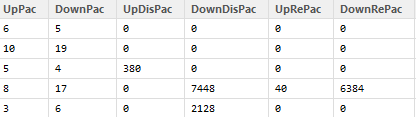
\includegraphics[width=0.7\linewidth]{images/11}
	\caption{Défaut de la système}
	\label{fig:défaut}
\end{figure}

Finalement nous avons décidé d'utiliser ces 5 attributs (la vitesse et le délai) pour mesurer la qualité du service.

\subsection{Les caractéristiques de données}



\begin{figure}[H]
\centering
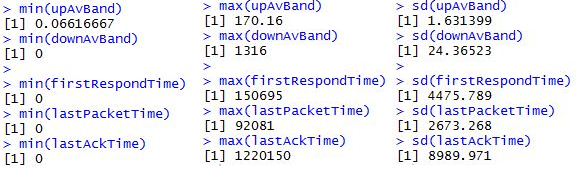
\includegraphics[width=0.8\linewidth, height=0.2\textheight]{images/max-min}
\caption{La valeur maximal, valeur minimal et l'écart type}
\label{fig:max-min}
\end{figure}

\begin{figure}[H]
\centering
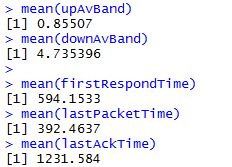
\includegraphics[width=0.3\linewidth]{images/mean}
\caption{La valeur moyenne}
\label{fig:mean}
\end{figure}

Nous avons trouvé que l'écart type pour les trois attributs de délais est très grand. Les valeurs varient de $0ms$ à $1220150ms$. Par contre le changement  de la vitesse de la liaison montante et descendante n'est pas très grand.

\begin{figure}[H]
\centering
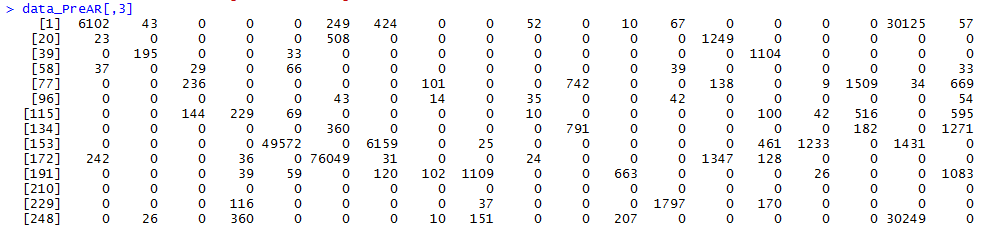
\includegraphics[width=0.9\linewidth]{images/data-delai}
\caption{Le temps de réponse du serveur}
\label{fig:data-delai}
\end{figure}
En analysant le données, nous avons trouvé que les données ne sont pas normal, et l'ingénieur du fournisseur de l'équipement nous ont confirmé que le système de collecte d'informations de signalisation a des défauts. 
 
%\section{La mise en \oe uvre}
\subsection{Le K-Means et Le Règle d'association }
\subsubsection{La valeur optimale de $k$}
Pour trouver le k optimal pour nos données, nous avons utilisé la technique 'silhouette C\oe fficient' et 'somme d'erreur carrés'.

Nous avons mesuré le résultat de ces deux techniques quand la valeur de $k$ augmente de $1$ à $15$, En tenant compte des caractéristiques de l'algorithme, pour chaque valeur de $k$, nous avons répété 50 fois en vue de calculer la valeur moyenne pour éliminer les erreurs. En suite, nous avons étudié le résultat pour trouver la valeur optimale.
\subsubsection*{La somme d'erreurs carrées}
\begin{figure}[H]
\centering
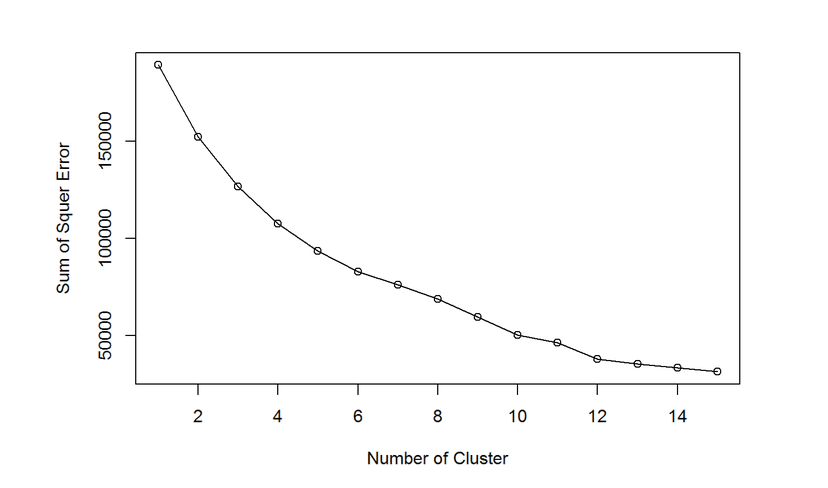
\includegraphics[width=0.8\linewidth]{images/sse}
\caption{somme d'erreur carrés}
\label{fig:sse}
\end{figure}
Nous avons trouvé que la somme d'erreurs carrées diminue quand $k$ augmente, mais il est difficile de choisir la valeur optimal de $k$ avec cette image.

\subsubsection*{La silhouette C\oe fficient}
Nous utilisons la même technique pour calculer et visualiser la valeur de la silhouette C\oe fficient en fonction de la valeur de $k$.

\begin{figure}[H]
\centering
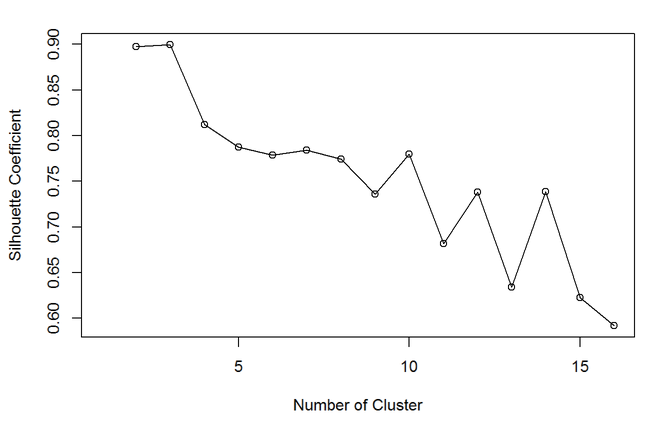
\includegraphics[width=0.9\linewidth]{images/sc}
\caption{la silhouette C\oe fficient quand k varie de 2 à 15}
\label{fig:sc}
\end{figure}

L'image de la silhouette C\oe fficient nous montrons que comme quand $k=3$ la valeur de la silhouette C\oe fficient est plus grandes. Donc nous soupçonnons que quand $k=3$ nous pouvons trouver le mieux partition.

\subsubsection{Le clustering}
Après classifie le données en 3 groupes utilisant l'algorithme CLARA. Nous avons trouvé que la majorité de données ($94 \%$ de données) sont dans le premier groupe, un groupe de $4,4 \%$, la troisième groupe a $1,6 \%$ de données.  

 \begin{figure}[H]
 	\flushleft
 	 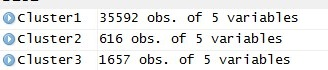
\includegraphics[width=0.45\linewidth]{images/3cluster}
 	 \label{fig:3cluster}
 	\hspace{1in}	 
 	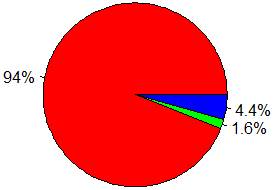
\includegraphics[width=0.325\linewidth]{images/piechart}
 	\label{fig:piechart}
 	\caption{Le nombre des trois clusters} 
 \end{figure}

En utilisant le fonction 'plot3d' fourni par le package 'rgl', nous pouvons visualiser le données en trois dimensions, et nous pouvons visualiser le résultat de clustering.


% bande passante moyenne de la liaison montante, bande passante moyenne de la liaison descendant, et le premier délai de réponse
\begin{figure}[H]
\centering
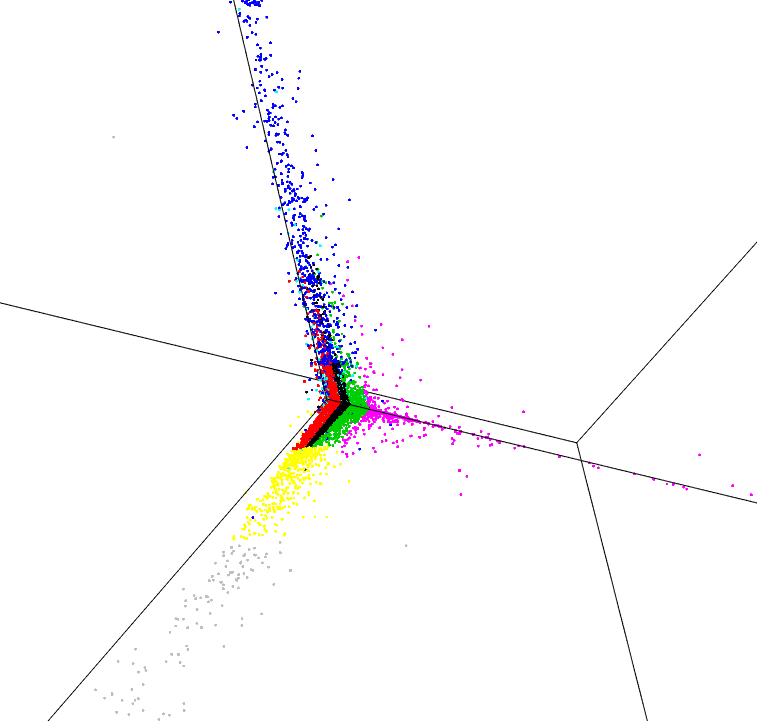
\includegraphics[width=0.6\linewidth]{images/kmeqn}
\caption{up link Average Band, down link Average Band, first Respond Time.}
\label{fig:kmeqn}
\end{figure}
\begin{figure}[H]
\centering
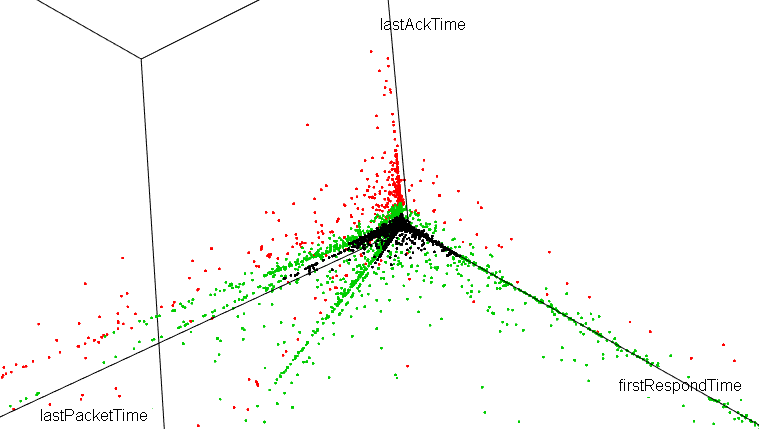
\includegraphics[width=0.8\linewidth]{images/3delai}
\caption{first Respond Time, last Packet Time, last Ack Time.}
\label{fig:3delai}
\end{figure}

Nous avons trouver que les points noir sont le données de 'cluster 1' , les points de 'cluster 2' sont en rouge, les points de 'cluster 3' sont en vert. 

Après le regroupement, nous pouvons utiliser l'algorithme 'k plus proches voisins' pour déterminer le nouveau données font partie de quel groupe .

\subsubsection{Le Règle d'association}
En utilisant le résultat de clustering, nous pouvons transformer le données numérique au données caractère. 

Nous y parvenons en quatre étapes
\begin{enumerate}
\item D'abord, nous trouvons les valeur minimal et maximal de chaque attribut\ref{fig:max-min1};
\item Ensuite, nous trouvons les intervalles de chaque attribut\ref{fig:seuil};
\item Puis, nous transformons le données numérique au données caractère\ref{fig:newData2};
\item \textsc{à} la fin, nous utilisons l'algorithme Apriori pour trouver des règles\ref{fig:newar}. 
\end{enumerate}
\begin{figure}[H]
\centering
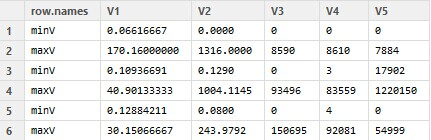
\includegraphics[width=0.8\linewidth]{images/max-min1}
\caption{trouver les valeur minimal et maximal de chaque attribut}
\label{fig:max-min1}
\end{figure}


\begin{figure}[H]
\centering
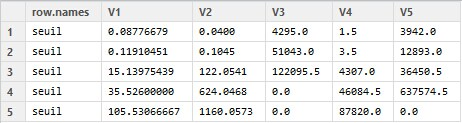
\includegraphics[width=0.8\linewidth]{images/seuil}
\caption{défini les intervalles}
\label{fig:seuil}
\end{figure}

\begin{figure}[H]
\centering
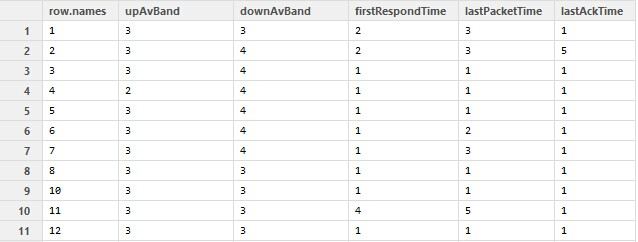
\includegraphics[width=0.8\linewidth]{images/newData2}
\caption{transformer les données numérique à données caractère}
\label{fig:newData2}
\end{figure}

En changeant les paramètres de l'algorithme, nous pouvons filtrer le résultat. Par exemple, nous cherchons les règles qui ont le support supérieur à
$0,5$ et la confidence supérieur à $0,8$, et aussi la valeur de 'lastAckTime' et 'upAvBand' sont dans la première intervalle\ref{fig:arp}. Et nous avons trouvé $7$ règle à la fin.\ref{fig:newar}

\begin{figure}[H]
\centering
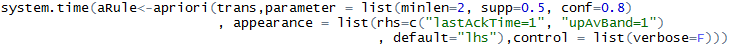
\includegraphics[width=1.2\linewidth]{images/arp}
\caption{L'algorithme règle d'association et le filtrage des données  }
\label{fig:arp}
\end{figure}


\begin{figure}[H]
\centering
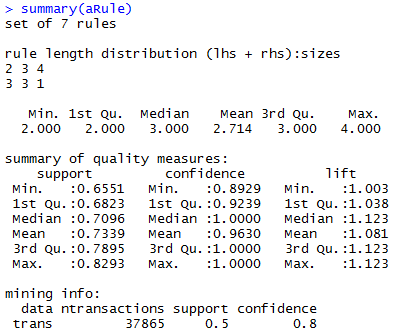
\includegraphics[width=0.5\linewidth]{images/ars}
\caption{Les règles trouvé par l'algorithme règle d'association  }
\label{fig:newar}
\end{figure}

\begin{figure}[H]
\centering
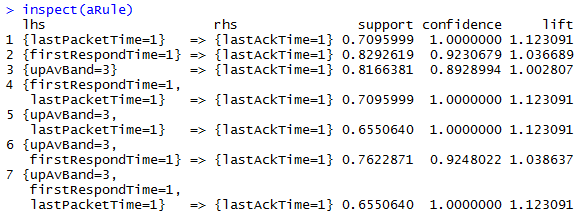
\includegraphics[width=0.8\linewidth]{images/AR2}
\caption{Les règles découvert}
\label{fig:AR2}
\end{figure}

Selon les règles trouvent par l'algorithme du Règle d'association, si la valeur de 'lastPacketTime' est dans la deuxième intervalle $1$ alors la valeur de 'lastAckTime' est plus susceptible d'être dans l'intervalle $1$, et entre tous les données ou la valeur de 'firstRespondTime' est dans la première intervalle, $.82,9\%$ d'entre eux la valeur de 'lastAckTime' est dans l'intervalle $1$.

En utilisant les paramètres différent, nous pouvons trouver le règle que nous avons besoin. Mais dans notre cas les règles trouvé ne sont pas clair.

\subsection{Le KmMST}
La deuxième méthode, nous utilisons l'algorithme K-Means avec MST.

Parce que l'algorithme K-Means ne fonctionne bien que avec les données de distribution sphérique, donc par clustering le données en beaucoup de partitions, et utilise la technique de MST, nous pouvons surmonter les défaut de K-Means et obtenir les bons résultats de clustering.
 
  \subsubsection{L'étape de l'algorithme KmMST}
  
  \begin{enumerate}
  \item Regroupement le données;\\
  
   La valeur de $K$ égal à $n^r$, le $n$ égal à la quantité de données, $r$ est dans l'intervalle de $0$ et $1$, par défaut, $r$ égal à $0,5$.
   
   En premier, nous avons regroupé le données en K partition.
   
  \item \textsc{é}tablir la matrice de distance;\\
  
  Après, nous pouvons utiliser les valeurs du centre de chaque partition pour calculer la matrice de distance
  \begin{figure}[H]
\centering
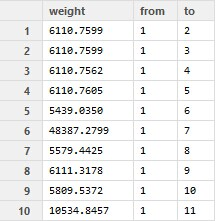
\includegraphics[width=0.4\linewidth]{images/distance}
\caption{la matrice de distance}
\label{fig:distance}
\end{figure}

  
  \item Utilise la technique de MST;\\
  
  \textsc{à} aide de la package 'igraph' nous pouvons trouver l'arbre couvrant de poids minimal.
  
  \begin{figure}[H]
\centering
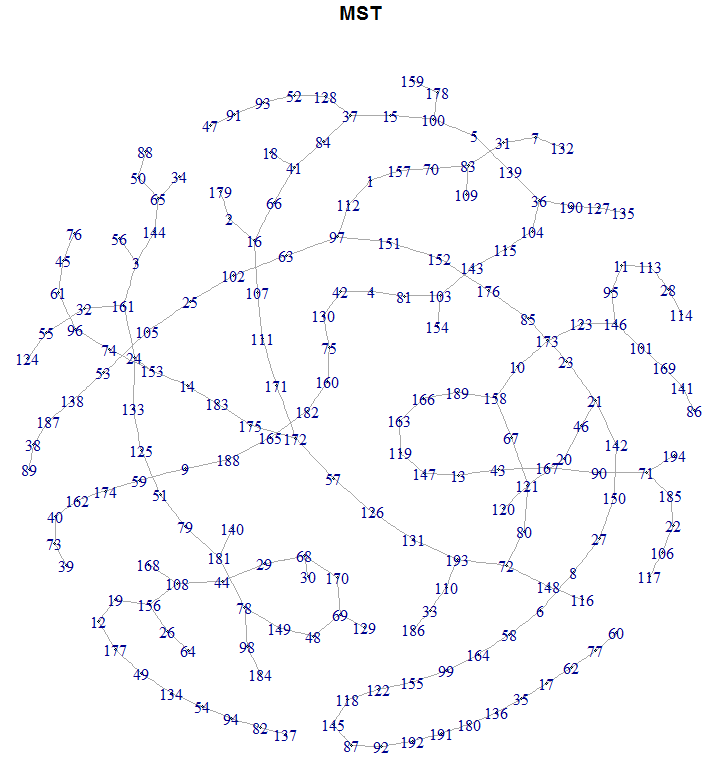
\includegraphics[width=0.45\linewidth]{images/mst2}
\caption{L'arbre couvrant de poids minimal}
\label{fig:mst2}
\end{figure}

  \item Coupe le arête le plus long
  
  Techniquement, nous pouvons trouver les partitions par couper les arête long, et nous avons tester avec différentes valeurs, mais les sommets sont devenu le point isolé.
  
  \begin{figure}[H]
\centering
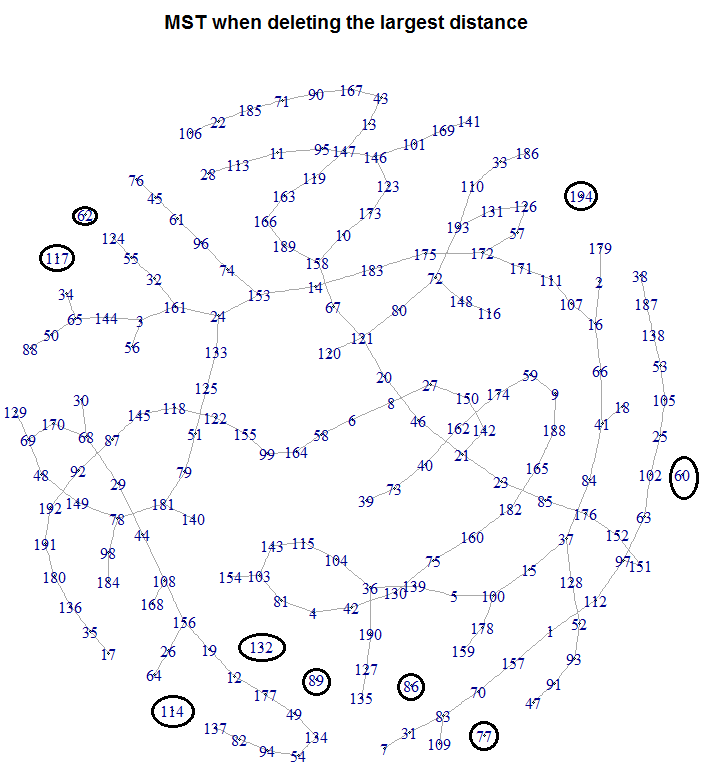
\includegraphics[width=0.6\linewidth]{images/mst10}
\caption{L'arbre couvrant de poids minimal, quand C = $10$}
\label{fig:mst10}
\end{figure}

  \end{enumerate}










